\begin{figure}[H]
    \begin{subfigure}[b]{0.3\textwidth}
        \centering
        \begin{lstlisting}
// hot path
if (cond)
coldFunc();
// hot path again\end{lstlisting}
        \caption{C Codes}
    \end{subfigure}
    \begin{subfigure}[b]{0.65\textwidth}
        \centering
        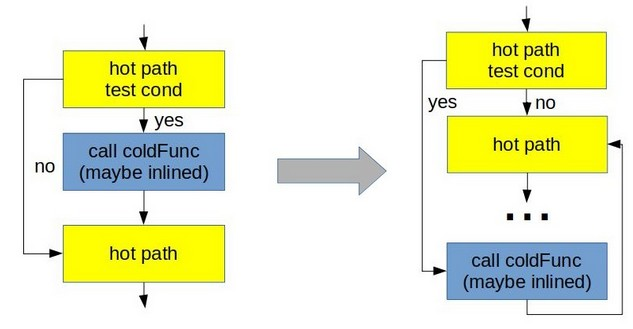
\includegraphics[width=0.86\textwidth]{images/hot_cold_placement.jpg}
        \caption{布局优化示例}
    \end{subfigure}
\end{figure}
\begin{itemize}
    \item 不进行分支跳转往往比跳转代价更低(maintain fall through)
    \item 更好地利用 Cache ($\mu$op-cache) (局部性)
\end{itemize}
